% I seguenti commenti speciali impostano:
% 1. 
% 2. PDFLaTeX come motore di composizione;
% 3. tesi.tex come documento principale;
% 4. il controllo ortografico italiano per l'editor.

% !TEX encoding = UTF-8
% !TEX TS-program = pdflatex
% !TEX root = tesi.tex
% !TEX spellcheck = it-IT

\documentclass[10pt,                    % corpo del font principale
               a4paper,                 % carta A4
               twoside,                 % impagina per fronte-retro
               openright,               % inizio capitoli a destra
               english,
               italian,
                ctexart,
               ]{book}

%**************************************************************
% Importazione package
%************************************************************** 
%\usepackage{amsmath,amssymb,amsthm}    % matematica
\usepackage[UTF8]{ctex}
\usepackage[T1]{fontenc}                % codifica dei font:
                                        % NOTA BENE! richiede una distribuzione *completa* di LaTeX

\usepackage[utf8]{inputenc}             % codifica di input; anche [latin1] va bene
                                        % NOTA BENE! va accordata con le preferenze dell'editor

\usepackage[english, italian]{babel}    % per scrivere in italiano e in inglese;
                                        % l'ultima lingua (l'italiano) risulta predefinita

\usepackage{bookmark}                   % segnalibri

\usepackage{caption}                    % didascalie

\usepackage{chngpage,calc}              % centra il frontespizio

\usepackage{csquotes}                   % gestisce automaticamente i caratteri (")

\usepackage{emptypage}                  % pagine vuote senza testatina e piede di pagina

\usepackage{epigraph}			% per epigrafi

\usepackage{eurosym}                    % simbolo dell'euro

%\usepackage{indentfirst}               % rientra il primo paragrafo di ogni sezione

\usepackage{graphicx}                   % immagini

\usepackage{hyperref}                   % collegamenti ipertestuali

\usepackage[binding=5mm]{layaureo}      % margini ottimizzati per l'A4; rilegatura di 5 mm

\usepackage{listings}                   % codici

\usepackage{microtype}                  % microtipografia

\usepackage{mparhack,fixltx2e,relsize}  % finezze tipografiche

\usepackage{nameref}                    % visualizza nome dei riferimenti                                      

\usepackage[font=small]{quoting}        % citazioni

%\usepackage{subfig}                     % sottofigure, sottotabelle

\usepackage[italian]{varioref}          % riferimenti completi della pagina

\usepackage[dvipsnames]{xcolor}         % colori
\usepackage{formattazione}

\usepackage{booktabs}                   % tabelle                                       
\usepackage{tabularx}                   % tabelle di larghezza prefissata                                    
\usepackage{longtable}                  % tabelle su più pagine                                        
\usepackage{ltxtable}                   % tabelle su più pagine e adattabili in larghezza

\usepackage[toc, acronym]{glossaries}   % glossario
                                        % per includerlo nel documento bisogna:
                                        % 1. compilare una prima volta tesi.tex;
                                        % 2. eseguire: makeindex -s tesi.ist -t tesi.glg -o tesi.gls tesi.glo
                                        % 3. eseguire: makeindex -s tesi.ist -t tesi.alg -o tesi.acr tesi.acn
                                        % 4. compilare due volte tesi.tex.

\usepackage[backend=biber,style=verbose-ibid,hyperref,backref]{biblatex}
                                        % eccellente pacchetto per la bibliografia;
                                        % produce uno stile di citazione autore-anno;
                                        % lo stile "numeric-comp" produce riferimenti numerici
                                        % per includerlo nel documento bisogna:
                                        % 1. compilare una prima volta tesi.tex;
                                        % 2. eseguire: biber tesi
                                        % 3. compilare ancora tesi.tex.

%**************************************************************
% file contenente le impostazioni della tesi
%**************************************************************

%**************************************************************
% Frontespizio
%**************************************************************

% Autore
\newcommand{\myName}{Xiaowei Wen}
\newcommand{\myTitle}{APAT - Android Platform Analysis Tool}

% Tipo di tesi                   
\newcommand{\myDegree}{Tesi di laurea triennale}

% Università             
\newcommand{\myUni}{Università degli Studi di Padova}

% Facoltà       
\newcommand{\myFaculty}{Corso di Laurea in Informatica}

% Dipartimento
\newcommand{\myDepartment}{Dipartimento di Matematica "Tullio Levi-Civita"}

% Titolo del relatore
\newcommand{\profTitle}{Prof.}

% Relatore
\newcommand{\myProf}{ Alessandro Sperduti}

% Luogo
\newcommand{\myLocation}{Padova}

% Anno accademico
\newcommand{\myAA}{2019-2020}

% Data discussione
\newcommand{\myTime}{23 Luglio 2020}


\addto\captionsitalian{\renewcommand{\lstlistingname}{Codice}}

%**************************************************************
% Impostazioni di impaginazione
% see: http://wwwcdf.pd.infn.it/AppuntiLinux/a2547.htm
%**************************************************************

\setlength{\parindent}{14pt}   % larghezza rientro della prima riga
\setlength{\parskip}{0pt}   % distanza tra i paragrafi


%**************************************************************
% Impostazioni di biblatex
%**************************************************************
\bibliography{bibliografia} % database di biblatex 

\defbibheading{bibliography} {
    \cleardoublepage
    \phantomsection 
    \addcontentsline{toc}{chapter}{\bibname}
    \chapter*{\bibname\markboth{\bibname}{\bibname}}
}

\setlength\bibitemsep{1.5\itemsep} % spazio tra entry

\DeclareBibliographyCategory{opere}
\DeclareBibliographyCategory{web}

\addtocategory{opere}{womak:lean-thinking}
\addtocategory{web}{site:agile-manifesto}

\defbibheading{opere}{\section*{Riferimenti bibliografici}}
\defbibheading{web}{\section*{Siti Web consultati}}


%**************************************************************
% Impostazioni di caption
%**************************************************************
\captionsetup{
    tableposition=top,
    figureposition=bottom,
    font=small,
    format=hang,
    labelfont=bf
}

%**************************************************************
% Impostazioni di glossaries
%**************************************************************
%**************************************************************
% Acronimi
%**************************************************************
\renewcommand{\acronymname}{Acronimi e abbreviazioni}
%**************************************************************

\newacronym[description={\glslink{apig}{Application Programming Interface}}]
{api}{API}{Application Programming Interface}
\newglossaryentry{apig}
{
name=\glslink{api}{API},
text= Application Programming Interface,
sort= api,
description={in informatica con il termine \emph{Application Programming Interface API} (ing. interfaccia di programmazione di un'applicazione) si indica ogni insieme di procedure disponibili al programmatore, di solito raggruppate a formare un set di strumenti specifici per l'espletamento di un determinato compito all'interno di un certo programma. La finalità è ottenere un'astrazione, di solito tra l'hardware e il programmatore o tra software a basso e quello ad alto livello semplificando così il lavoro di programmazione}
}
%**************************************************************

\newacronym[description={\glslink{umlg}{Unified Modelling Language}}]
{uml}{UML}{Unified Modelling Language}
\newglossaryentry{umlg}
{
name=\glslink{uml}{UML},
text= Unified Modelling Language,
sort= UML,
description={In ingegneria del software \emph{UML, Unified Modeling Language} (ing. linguaggio di modellazione unificato) è un linguaggio di modellazione e specifica basato sul paradigma object-oriented. L'\emph{UML} svolge un'importantissima funzione di ``lingua franca'' nella comunità della progettazione e programmazione a oggetti. Gran parte della letteratura di settore usa tale linguaggio per descrivere soluzioni analitiche e progettuali in modo sintetico e comprensibile a un vasto pubblico}
}

%**************************************************************

\newacronym[description={\glslink{dexg}{Dalvik Executable}}]
{dex}{DEX}{Dalvik Executable}
\newglossaryentry{dexg}
{
name=\glslink{dex}{DEX},
text= Dalvik Executable,
sort= dex,
description={File eseguibili Dalvik sono file di sviluppo apposte con il .dex estensione, e questi file DEX vengono utilizzati per inizializzare ed eseguire applicazioni sviluppate per il sistema operativo mobile Android.
I dati memorizzati in questi file DEX include compilato il codice che individua e inizializza altri file di programma dell'applicazione associata necessario per eseguire il programma}
}
%**************************************************************

\newacronym[description={\glslink{apkg}{Android Package}}]
{apk}{APK}{ Android Package }
\newglossaryentry{apkg}
{
name=\glslink{apk}{APK},
text= Android Package,
sort= apk,
description={L'estensione APK indica un file Android Package.
Questo formato di file, una variante del formato .JAR, è utilizzato per la distribuzione e l'installazione di componenti in dotazione sulla piattaforma per dispositivi mobili Android}
}
%**************************************************************

\newacronym[description={\glslink{kissg}{Keep It Simple Stupid}}]
{kiss}{KISS}{Keep It Simple Stupid}
\newglossaryentry{kissg}
{
name=\glslink{kiss}{KISS},
text= Keep It Simple Stupid,
sort= kiss,
description={Il principio utilizzato nel mondo dell'informatica per indicare maggior parte dei sistemi semplici hanno una prestazione maggiore rispetto ai sistemi complicati.
Anche se, la semplicità deve essere un obiettivo da perseguire nella progettazione e la complessità aggiuntiva non necessaria deve essere evitata}
}
%**************************************************************

\newacronym[description={\glslink{scag}{Software Component Analysis}}]
{sca}{SCA}{ Software Component Analysis }
\newglossaryentry{scag}
{
name=\glslink{sca}{SCA},
text= Software Component Analysis,
sort= sca,
description={Software Component Analysis è una parte dell'industria del software relativamente nuova. Questi strumenti sono spesso costruiti assemblando componenti terze parti o open-source, integrate con codice con il codice orginale.\footcite{site:sca}}
}
%**************************************************************

\newacronym[description={\glslink{sastg}{Static Application Security Testing}}]
{sast}{SAST}{ Static Application Security Testing }
\newglossaryentry{sastg}
{
name=\glslink{sast}{SAST},
text= Static Application Security Testing,
sort= sast,
description={Static Application Security Testing\footcite{site:sast} è una tecnologia che è frequentemente utilizzato come un tool di analisi del codice sorgente. Il metodo analizza il codice sorgente dal punto di vista della vulnerabilità anche se potrebbe produrre alcuni falsi positivi ma per la maggior parte delle implementazioni richiede l'accesso al codice sorgente, complicate configurazioni e alta potenza di calcolo.}
}

%**************************************************************

\newacronym[description={\glslink{dastg}{Dynamic Application Security Testing}}]
{dast}{DAST}{Dynamic Application Security Testing}
\newglossaryentry{dastg}
{
name=\glslink{dast}{DAST},
text= Dynamic Application Security Testing,
sort= dast,
description={Dynamic APplication Security Testing è una tecnologia che è capace di trovare vulnerabilità eseguendo l'applicazione. Questo metodo è altamente scalabile, facilmente e velocemente integrabile. Il punto debole del DAST è che ha bisogno della configurazione esperta e potrebbe produrre sia falsi positivi che negativi.}
}

%**************************************************************

\newacronym[description={\glslink{ideg}{Integrated Development Environment}}]
{ide}{IDE}{Integrated Development Environment}
\newglossaryentry{ideg}
{
name=\glslink{ide}{IDE},
text=Integrated Development Environment,
sort=ide,
description={ è un software che, in fase di programmazione, aiuta i programmatori nello sviluppo del codice sorgente di un programma.
Spesso l’IDE aiuta lo sviluppatore segnalando errori di sintassi del codice direttamente nella fase di scrittura, oltre a tutta una serie di strumenti e funzionalità di supporto alla fase di sviluppo e debugging}
}

%**************************************************************

\newacronym[description={\glslink{avdg}{Android Virtual Device}}]
{avd}{AVD}{Android Virtual Device}
\newglossaryentry{avdg}
{
name=\glslink{avd}{AVD},
text= Android Virtual Device,
sort= avd,
description={è una macchina virtuale fornito da Google che permette di avere un'istanza di qualsiasi versione del sistema operativo Android in esecuzione nei computer per poter testare le applicazioni android senza dover utilizzare uno smartphone}
}

%**************************************************************

\newacronym[description={\glslink{apatg}{Android Package Analysis Tool}}]
{apat}{APAT}{Android Package Analysis Tool}
\newglossaryentry{apatg}
{
name=\glslink{apat}{APAT},
text= Android Package Analysis Tool,
sort= apat,
description={è un tool che, dato un file APK, può effettuare una serie di operazioni di decompilazioni, decodifica, ricompilazione e l'analisi del codice sorgente generando al termine un file di report}
}

%**************************************************************

\newacronym[description={\glslink{slocg}{Source Line Of Code}}]
{sloc}{SLOC}{Source Line Of Code}
\newglossaryentry{slocg}
{
name=\glslink{sloc}{SLOC},
text= Source Line Of Code,
sort= Source Line Of Code,
description={è una metrica software che misura le dimensioni di un software basandosi sul numero di linee di codice sorgente.
Questo metodo di misura viene utilizzato per stabilire la complessità di un software e per stimare le risorse necessarie per la produzione e il mantenimento del software.
Se il software è di grandi dimensioni, possono essere utilizzate anche le unità di misura KLOC (1 000 LOC) e MLOC (1 000 000 LOC)}
}

%**************************************************************
%\newacronym[description={\glslink{testoConG}{TestoXEsteso}}]
%{TESTO_DA_CATTURARE}{ACRONIMO}{TestoXEsteso}
%\newglossaryentry{testoConG}
%{
%name=\glslink{TESTO_DA_CATTURARE}{ACRONIMO},
%text= TestoXEsteso,
%sort= TESTO_DA_ORDINARE,
%description={Descrizoine}
%}
%\newacronym[description={\glslink{testoConG}{TestoXEsteso}}]
%{TESTO_DA_CATTURARE}{ACRONIMO}{TestoXEsteso}
%\newglossaryentry{testoConG}
%{
%name=\glslink{TESTO_DA_CATTURARE}{ACRONIMO},
%text= TestoXEsteso,
%sort= TESTO_DA_ORDINARE,
%description={Descrizoine}
%}
%\newacronym[description={\glslink{testoConG}{TestoXEsteso}}]
%{TESTO_DA_CATTURARE}{ACRONIMO}{TestoXEsteso}
%\newglossaryentry{testoConG}
%{
%name=\glslink{TESTO_DA_CATTURARE}{ACRONIMO},
%text= TestoXEsteso,
%sort= TESTO_DA_ORDINARE,
%description={Descrizoine}
%}
%\newacronym[description={\glslink{testoConG}{TestoXEsteso}}]
%{TESTO_DA_CATTURARE}{ACRONIMO}{TestoXEsteso}
%\newglossaryentry{testoConG}
%{
%name=\glslink{TESTO_DA_CATTURARE}{ACRONIMO},
%text= TestoXEsteso,
%sort= TESTO_DA_ORDINARE,
%description={Descrizoine}
%}


%**************************************************************
% Glossario
%**************************************************************
%\renewcommand{\glossaryname}{Glossario}



\newglossaryentry{repackaging}
{
name=\glslink{repackaging}{repackaging},
text=repackaging,
sort=repackaging,
description={in ingegneria del software, il termine repackaging indica il processo di creazione del pacchetto d'installazione a seguito di un processo di trasformazione contraria}
}

\newglossaryentry{pcap}
{
name=\glslink{pcap}{pcap},
text=pcap,
sort=pcap,
description={I file con estensione .pcap contengono dati acquisiti dai programmi di tracciamento del pacchetto di trasmissione dati.
I dati sono in forma grezza, il che significa esattamente la stessa forma in cui è stato catturato.
I file sono spesso definiti come file di traccia o file ossei.
Salvare i pacchetti catturati usando il formato pcap può essere fatto da molti tipi di app, chiamati sniffer.
Questi programmi quindi analizzano i dati acquisiti come richiesto dall'utente, applicando la filtrazione e l'elaborazione appropriate.}
}
\newglossaryentry{walkthrough}
{
name=\glslink{walkthrough}{Walkthrough},
text=walkthrough,
sort=walkthrough,
description={è una pratica dell’analisi statica che viene usata per rivelare la presenza di difetti.
Richiede la rilettura ad ampio spettro del codice con attenzione, senza discriminare le parti meno significative}
}
\newglossaryentry{inspection}
{
name=\glslink{inspection}{Inspection},
text=inspection,
sort=inspection,
description={Inspection è una pratica dell’analisi statica che viene usata per rivelare la presenza di difetti.
Questa ricerca viene fatta in modo mirato solitamente in seguito al presentarsi di un errore, per poter effettura l'inspection bisogna aver prima stilato una lista di controllo che contiene i punti del codice con più probabilità di contenere un errore, inoltre, l'aggiornamento di quest'ultima è estremamente importante}
}
\newglossaryentry{ciclomatica}
{
name=\glslink{ciclomatica}{complessità ciclomatica},
text=complessità ciclomatica,
sort=complessità ciclomatica,
description={è una metrica utilizzata per misurare la complessità di un programma.
Misura direttamente il numero di cammini linearmente indipendenti attraverso il grafo di controllo di flusso.
La complessità ciclomatica è calcolata utilizzando il grafo di controllo di flusso del programma: i nodi del grafo corrispondono a gruppi indivisibili d'istruzioni, mentre gli archi connettono due nodi se il secondo gruppo d'istruzioni può essere eseguito immediatamente dopo il primo gruppo.
La complessità ciclomatica può, inoltre, essere applicata a singole funzioni, moduli, metodi o classi di un programma.\cite{site:complessita_ciclomatica} }
}
\newglossaryentry{buildautomation}
{
name=\glslink{buildautomation}{Build automation},
text=build automation,
sort=build automation,
description={è il processo di automatizzazione della creazione del build software e i processi inclusi sono: compilazione del codice sorgente in codice binario, packaging del codice binario ed esecuzione dei test automatici}
}

\newglossaryentry{codecoverage}
{
name=\glslink{codecoverage}{code coverage},
text=code coverage,
sort=code coverage,
description={è la metrica utilizzata per descrivere il grado con il quale il codice sorgente è stato eseguito dai test.
Un programma con un'alta percentuale di code coverage è meno probabile che contenga degli errori.}
}
\newglossaryentry{swing}
{
name=\glslink{swing}{swing},
text=Swing,
sort=swing,
description={è una libreria di Java che permette di creare interfaccia grafica}
}
\newglossaryentry{reverse_engineering}
{
name=\glslink{reverse_engineering}{reverse engineering},
text=Reverse engineering,
sort=reverseengineering,
description={è una tecnica di analisi delle funzioni, degli impieghi, della collocazione, dell'aspetto progettuale, geometrico e materiale di un manufatti i di un oggetto che è stato rivenuto.
Lo scopo è quello di produrre un altro oggetto che abbia un funzionamento analogo o migliore, o più adatto al contesto in cui ci si trova}
}
\newglossaryentry{xml}
{
name=\glslink{xml}{XML},
text=XML,
sort=XML,
description={ (acronimo di eXtensible Markup Language) è un metalinguaggio per la definizione dei linguaggi di markup, ovvero un linguaggio marcatore basato su un meccanismo sintattico che consente di definire e controllare il significato degli elementi contenuti in un documento o in un testo.
Il nome indica che si tratta di un linguaggio marcatore estendibile, in quanto permettere di creare tag personalizzati.}
}
\newglossaryentry{android_studio}
{
    name=\glslink{android_studio}{Android Studio},
    text=Android Studio,
    sort=Android Studio,
    description={è l'IDE ufficiale sviluppato e mantenuto da Google Inc.
\`{E} basato sul software di JetBrains Intellij IDEA ed è progettato specificamente per lo sviluppo di applicazioni Android.
Nasce per sostituire gli Android Development Tools (ADT) di Eclipse.}
}
%\newglossaryentry{}
%{
%    name=\glslink{}{},
%    text=,
%    sort=,
%    description={}
%}
%\newglossaryentry{}
%{
%    name=\glslink{}{},
%    text=,
%    sort=,
%    description={}
%}
%\newglossaryentry{}
%{
%    name=\glslink{}{},
%    text=,
%    sort=,
%    description={}
%}
%\newglossaryentry{}
%{
%    name=\glslink{}{},
%    text=,
%    sort=,
%    description={}
%}
%\newglossaryentry{}
%{
%    name=\glslink{}{},
%    text=,
%    sort=,
%    description={}
%}
%\newglossaryentry{}
%{
%    name=\glslink{}{},
%    text=,
%    sort=,
%    description={}
%}
%\newglossaryentry{}
%{
%    name=\glslink{}{},
%    text=,
%    sort=,
%    description={}
%}
%\newglossaryentry{}
%{
%    name=\glslink{}{},
%    text=,
%    sort=,
%    description={}
%}
%\newglossaryentry{}
%{
%    name=\glslink{}{},
%    text=,
%    sort=,
%    description={}
%}

 % database di termini
\makeglossaries


%**************************************************************
% Impostazioni di graphicx
%**************************************************************
\graphicspath{{immagini/}} % cartella dove sono riposte le immagini


%**************************************************************
% Impostazioni di hyperref
%**************************************************************
\hypersetup{
    %hyperfootnotes=false,
    %pdfpagelabels,
    %draft,	% = elimina tutti i link (utile per stampe in bianco e nero)
    colorlinks=true,
    linktocpage=true,
    pdfstartpage=1,
    pdfstartview=FitV,
    % decommenta la riga seguente per avere link in nero (per esempio per la stampa in bianco e nero)
    %colorlinks=false, linktocpage=false, pdfborder={0 0 0}, pdfstartpage=1, pdfstartview=FitV,
    breaklinks=true,
    pdfpagemode=UseNone,
    pageanchor=true,
    pdfpagemode=UseOutlines,
    plainpages=false,
    bookmarksnumbered,
    bookmarksopen=true,
    bookmarksopenlevel=1,
    hypertexnames=true,
    pdfhighlight=/O,
    %nesting=true,
    %frenchlinks,
    urlcolor=webbrown,
    linkcolor=RoyalBlue,
    citecolor=webgreen,
    %pagecolor=RoyalBlue,
    %urlcolor=Black, linkcolor=Black, citecolor=Black, %pagecolor=Black,
    pdftitle={\myTitle},
    pdfauthor={\textcopyright\ \myName, \myUni, \myFaculty},
    pdfsubject={},
    pdfkeywords={},
    pdfcreator={pdfLaTeX},
    pdfproducer={LaTeX}
}

%**************************************************************
% Impostazioni di itemize
%**************************************************************
%\renewcommand{\labelitemi}{$\ast$}

%\renewcommand{\labelitemi}{$\bullet$}
%\renewcommand{\labelitemii}{$\cdot$}
%\renewcommand{\labelitemiii}{$\diamond$}
%\renewcommand{\labelitemiv}{$\ast$}


%**************************************************************
% Impostazioni di listings
%**************************************************************
\lstset{
    language=[LaTeX]Tex,%C++,
    keywordstyle=\color{RoyalBlue}, %\bfseries,
    basicstyle=\small\ttfamily,
    %identifierstyle=\color{NavyBlue},
    commentstyle=\color{Green}\ttfamily,
    stringstyle=\rmfamily,
    numbers=none, %left,%
    numberstyle=\scriptsize, %\tiny
    stepnumber=5,
    numbersep=8pt,
    showstringspaces=false,
    breaklines=true,
    frameround=ftff,
    frame=single
} 


%**************************************************************
% Impostazioni di xcolor
%**************************************************************
\definecolor{webgreen}{rgb}{0,.5,0}
\definecolor{webbrown}{rgb}{.6,0,0}
\usepackage{chngcntr}
\counterwithout{footnote}{chapter}

%**************************************************************
% Altro
%**************************************************************

\newcommand{\omissis}{[\dots\negthinspace]} % produce [...]

% eccezioni all'algoritmo di sillabazione
\hyphenation
{
    ma-cro-istru-zio-ne
    gi-ral-din
}

\newcommand{\sectionname}{sezione}
\addto\captionsitalian{\renewcommand{\figurename}{Figura}
                       \renewcommand{\tablename}{Tabella}}

\newcommand{\glsfirstoccur}{\ap{{[g]}}}

\newcommand{\intro}[1]{\emph{\textsf{#1}}}

%**************************************************************
% Environment per ``rischi''
%**************************************************************
\newcounter{riskcounter}                % define a counter
\setcounter{riskcounter}{0}             % set the counter to some initial value

%%%% Parameters
% #1: Title
\newenvironment{risk}[1]{
    \refstepcounter{riskcounter}        % increment counter
    \par \noindent                      % start new paragraph
    \textbf{\arabic{riskcounter}. #1}   % display the title before the 
                                        % content of the environment is displayed 
}{
    \par\medskip
}

\newcommand{\riskname}{Rischio}

\newcommand{\riskdescription}[1]{\textbf{\\Descrizione:} #1.}

\newcommand{\risksolution}[1]{\textbf{\\Soluzione:} #1.}

%**************************************************************
% Environment per ``use case''
%**************************************************************
\newcounter{usecasecounter}             % define a counter
\setcounter{usecasecounter}{0}          % set the counter to some initial value

%%%% Parameters
% #1: ID
% #2: Nome
\newenvironment{usecase}[2]{
    \renewcommand{\theusecasecounter}{\usecasename #1}  % this is where the display of 
                                                        % the counter is overwritten/modified
    \refstepcounter{usecasecounter}             % increment counter
    \vspace{10pt}
    \par \noindent                              % start new paragraph
    {\large \textbf{\usecasename #1: #2}}       % display the title before the 
                                                % content of the environment is displayed 
    \medskip
}{
    \medskip
}

\newcommand{\usecasename}{UC}

\newcommand{\usecaseactors}[1]{\textbf{\\Attori Principali:} #1. \vspace{4pt}}
\newcommand{\usecasepre}[1]{\textbf{\\Precondizioni:} #1. \vspace{4pt}}
\newcommand{\usecasedesc}[1]{\textbf{\\Descrizione:} #1. \vspace{4pt}}
\newcommand{\usecasepost}[1]{\textbf{\\Postcondizioni:} #1. \vspace{4pt}}
\newcommand{\usecasealt}[1]{\textbf{\\Scenario Alternativo:} #1. \vspace{4pt}}

%**************************************************************
% Environment per ``namespace description''
%**************************************************************

\newenvironment{namespacedesc}{
    \vspace{10pt}
    \par \noindent                              % start new paragraph
    \begin{description} 
}{
    \end{description}
    \medskip
}

\newcommand{\classdesc}[2]{\item[\textbf{#1:}] #2}
\renewcommand{\labelitemi}{$\bullet$}
\renewcommand{\labelitemii}{$\circ$}
\renewcommand{\labelitemiii}{-}
\renewcommand{\labelitemiv}{$\cdot$}
                     % file con le impostazioni personali

\begin{document}
%**************************************************************
% Materiale iniziale
%**************************************************************
\frontmatter
% !TEX encoding = UTF-8
% !TEX TS-program = pdflatex
% !TEX root = ../tesi.tex

%**************************************************************
% Frontespizio 
%**************************************************************
\begin{titlepage}

\begin{center}

\begin{LARGE}
\textbf{\myUni}\\
\end{LARGE}

\vspace{10pt}

\begin{Large}
\textsc{\myDepartment}\\
\end{Large}

\vspace{10pt}

\begin{large}
\textsc{\myFaculty}\\
\end{large}

\vspace{30pt}
\begin{figure}[htbp]
\begin{center}

\includegraphics[height=6cm]{logo-unipd}
\end{center}
\end{figure}
\vspace{30pt} 

\begin{LARGE}
\begin{center}
\textbf{\myTitle}\\
\end{center}
\end{LARGE}

\vspace{10pt} 

\begin{large}
\textsl{\myDegree}\\
\end{large}

\vspace{40pt}

\begin{large}
\begin{flushleft}
\textit{Relatore}\\ 
\vspace{5pt} 
\profTitle \myProf
\end{flushleft}

\vspace{0pt} 

\begin{flushright}
\textit{Laureando}\\ 
\vspace{5pt} 
\myName
\end{flushright}
\end{large}

\vspace{20pt}

\line(1, 0){338} \\
\begin{normalsize}
\textsc{Anno Accademico \myAA}
\end{normalsize}

\end{center}
\end{titlepage} 
% !TEX encoding = UTF-8
% !TEX TS-program = pdflatex
% !TEX root = ../tesi.tex

%**************************************************************
% Colophon
%**************************************************************
\clearpage
\phantomsection
\thispagestyle{empty}

\hfill

\vfill

\noindent\myName: \textit{\myTitle,}
\myDegree,
\textcopyright\ \myTime.
% !TEX encoding = UTF-8
% !TEX TS-program = pdflatex
% !TEX root = ../tesi.tex

%**************************************************************
% Dedica
%**************************************************************
\cleardoublepage
\phantomsection
\thispagestyle{empty}
\pdfbookmark{Dedica}{Dedica}

\vspace*{3cm}

\begin{center}
    但愿日子清净, 抬头遇见的都是柔情.\\ \medskip
    "Così come in algebra due affermazioni false ne danno una vera, così spero che il prodotto dei miei insuccessi si concluda con un successo." \medskip
    --V. Van Gogh
\end{center}

\medskip

\begin{center}
Dedicato a nonna Giovanna e a tutte le persone che mi hanno aiutato per essere qui.
\end{center}

% !TEX encoding = UTF-8
% !TEX TS-program = pdflatex
% !TEX root = ../tesi.tex

%**************************************************************
% Sommario
%**************************************************************
\cleardoublepage
\phantomsection
\pdfbookmark{Sommario}{Sommario}
\begingroup
\let\clearpage\relax
\let\cleardoublepage\relax
\let\cleardoublepage\relax

\chapter*{Sommario}

Il presente documento descrive il lavoro svolto durante il periodo di stage, della durata di circa trecento ore, dal laureando Xiaowei Wen presso l'azienda Imola Informatica S.p.A. Gli obbiettivi da raggiungere erano molteplici. In primo luogo era richiesto lo sviluppo di un tool in grado di automatizzare la decompilazione di un file \textit{APK} e la ricompilazione del file. In secondo luogo era richiesta l'implementazione di alcune funzionalità di analisi del codice sorgente ottenuto dal passo precedente.
Terzo e ultimo obbiettivo era quello di permettere di eseguire l'app con il proxy in un AVD e di monitorare il traffico di rete generando un file \textit{cap}.

%\vfill
%
%\selectlanguage{english}
%\pdfbookmark{Abstract}{Abstract}
%\chapter*{Abstract}
%
%\selectlanguage{italian}

\endgroup			

\vfill


% !TEX encoding = UTF-8
% !TEX TS-program = pdflatex
% !TEX root = ../tesi.tex

%**************************************************************
% Ringraziamenti
%**************************************************************
\cleardoublepage
\phantomsection
\pdfbookmark{Ringraziamenti}{ringraziamenti}
\begin{flushright}{
	\slshape
	``Dio benedica quelle persone che quando incroci il loro sguardo per sbaglio, sorridono.''} \\
	\medskip
\end{flushright}


\bigskip

\begingroup
\let\clearpage\relax
\let\cleardoublepage\relax
\let\cleardoublepage\relax

\chapter*{Ringraziamenti}

\noindent \textit{Innanzitutto, vorrei esprimere la mia gratitudine al Prof. Sperduti, relatore della mia tesi, e Alessandro Proscia, il tutor aziendale, per l'aiuto e il sostegno fornitomi durante la stesura del lavoro.}\\

\noindent \textit{Desidero ringraziare con affetto i miei genitori per il sostegno, il grande aiuto e per essermi stati vicini in ogni momento durante gli anni di studio.}\\

\noindent \textit{Ho desiderio di ringraziare poi Veronica, Alberto, Marco, Lorenzo, Linpeng, Tommaso, Alessandro e Giulio per tutti i bellissimi anni passati insieme, le avventure vissute e di essersi sorbiti mille delle mie lamentele.}\\

\noindent \textit{Infine, vorrei esprimere la mia gratitudine alla famiglia Geminian e Bernardi per tutti gli aiuti ricevuti durante questi anni.}\\
\bigskip

\noindent\textit{\myLocation, \myTime}
\hfill \myName

\endgroup


% !TEX encoding = UTF-8
% !TEX TS-program = pdflatex
% !TEX root = ../tesi.tex

%**************************************************************
% Indici
%**************************************************************
\cleardoublepage
\pdfbookmark{\contentsname}{tableofcontents}
\setcounter{tocdepth}{2}
\tableofcontents
%\markboth{\contentsname}{\contentsname} 
\clearpage

\begingroup 
    \let\clearpage\relax
    \let\cleardoublepage\relax
    \let\cleardoublepage\relax
    %*******************************************************
    % Elenco delle figure
    %*******************************************************    
    \phantomsection
    \pdfbookmark{\listfigurename}{lof}
    \listoffigures

    \vspace*{8ex}

    %*******************************************************
    % Elenco delle tabelle
    %*******************************************************
    \phantomsection
    \pdfbookmark{\listtablename}{lot}
    \listoftables
    \vspace*{8ex}
\endgroup

\cleardoublepage

\cleardoublepage

%**************************************************************
% Materiale principale
%**************************************************************
\mainmatter
% !TEX encoding = UTF-8
% !TEX TS-program = pdflatex
% !TEX root = ../tesi.tex

%**************************************************************
\chapter{Introduzione}\label{ch:introduzione}
%**************************************************************

Introduzione al contesto applicativo.\\

\noindent Esempio di utilizzo di un termine nel glossario \\
\gls{api}. \\

\noindent Esempio di citazione in linea \\
\cite{site:agile-manifesto}. \\

\noindent Esempio di citazione nel pie' di pagina \\
citazione\footcite{womak:lean-thinking} \\

%**************************************************************
\section{L'azienda}

Descrizione dell'azienda.

%**************************************************************
\section{L'idea}

Introduzione all'idea dello stage.

%**************************************************************
\section{Organizzazione del testo}

\begin{description}
    \item[{\hyperref[cap:processi-metodologie]{Il secondo capitolo}}] descrive ...
    
    \item[{\hyperref[cap:descrizione-stage]{Il terzo capitolo}}] approfondisce ...
    
    \item[{\hyperref[cap:analisi-requisiti]{Il quarto capitolo}}] approfondisce ...
    
    \item[{\hyperref[cap:progettazione-codifica]{Il quinto capitolo}}] approfondisce ...
    
    \item[{\hyperref[cap:verifica-validazione]{Il sesto capitolo}}] approfondisce ...
    
    \item[{\hyperref[cap:conclusioni]{Nel settimo capitolo}}] descrive ...
\end{description}

Riguardo la stesura del testo, relativamente al documento sono state adottate le seguenti convenzioni tipografiche:
\begin{itemize}
	\item gli acronimi, le abbreviazioni e i termini ambigui o di uso non comune menzionati vengono definiti nel glossario, situato alla fine del presente documento;
	\item per la prima occorrenza dei termini riportati nel glossario viene utilizzata la seguente nomenclatura: \emph{parola}\glsfirstoccur;
	\item i termini in lingua straniera o facenti parti del gergo tecnico sono evidenziati con il carattere \emph{corsivo}.
\end{itemize}             % Introduzione
% !TEX encoding = UTF-8
% !TEX TS-program = pdflatex
% !TEX root = ../tesi.tex

%**************************************************************
\chapter{Processi e metodologie}
\label{cap:processi-metodologie}
%**************************************************************

\intro{Brevissima introduzione al capitolo}\\

%**************************************************************
\section{Processo sviluppo prodotto}             % Processi
% !TEX encoding = UTF-8
% !TEX TS-program = pdflatex
% !TEX root = ../tesi.tex

%**************************************************************
\chapter{Descrizione dello stage}
\label{ch:descrizione-stage}
%**************************************************************

\intro{Questo capito contiene l'introduzione del progetto, l'analisi dei rischi, la specifica degli obiettivi e la pianificazione dei lavori.}\\

%**************************************************************
\section{Introduzione al progetto}\label{sec:introduzione-al-progetto}
Le applicazioni mobili rappresentano oggi una delle principali sfide per la sicurezza informatica: negli ultimi anni se la rapida diffusione degli smartphone ha visto emergere il mobile come uno dei principali canali per l'erogazione di servizi, sono aumentati esponenzialmente gli attacchi contro le piattaforme mobili.

Le applicazioni mobili soffrono spesso di debolezze intrinseche dovute al design dell'applicazione e al suo sviluppo, debolezze che possono prevedere la memorizzazione d'informazioni sensibili sul device, possibilità di modificare l'applicazione (mediante \gls{repackaging} dell'App), o la possibilità di un semplice reverse engineering.

Minacce tipiche dell'ambiente mobile sono:
\begin{itemize}
    \setlength\itemsep{0.1em}
    \item Utilizzo improprio della piattaforma
    \item Archiviazione dei dati non sicura
    \item Comunicazione insicura
    \item Autenticazione non sicura
\end{itemize}

%**************************************************************
\section{Analisi preventiva dei rischi}\label{sec:analisi-preventiva-dei-rischi}

Durante la fase di analisi iniziale sono stati individuati alcuni possibili rischi a cui si potrà andare incontro.
Si è quindi proceduto a elaborare delle possibili soluzioni per far fronte a tali rischi.\\

\begin{risk}{Tecnologie/framework sconosciute}
    \riskdescription{Durante lo svolgimento dello stage, sono richieste l'uso di alcune tecnologie o di framework fin'ora mai viste dallo stagista.}
    \risksolution{\`{E} stato programmato un periodo di auto-formazione riguardanti le tecnologie che si prevede di utilizzare, inoltre, il tutor aziendale si è reso disponibile di aiutare lo stagista se necessario}
    \label{risk:tecnologie-framework-sconosciute}
\end{risk}

%**************************************************************
\section{Requisiti e obiettivi}\label{sec:requisiti-e-obiettivi}
Lo scopo dello stage è la realizzazione di un tool di analisi di applicazioni Android che permetta di automatizzare operazioni di reverse engineering dei pacchetti delle app mobile (APK), effettuando nell'ordine:
\begin{enumerate}
    \setlength\itemsep{0.1em}
    \item decompilazione sorgenti;
    \item \gls{repackaging} dell'applicativo.
\end{enumerate}

Al termine dell'esecuzione dovranno essere rese disponibili informazioni quali:
\begin{itemize}
    \setlength\itemsep{0.1em}
    \item sorgenti decompilati;
    \item stringhe estratte dai sorgenti per l'individuazione di chiavi hard coded;
    \item contenuto della storage area dell'app;
    \item stringhe estratte dalla storage area dell'app per l'inviduazione d'informazioni sensibili;
    \item file di trace per le operazioni di rete effettuate (come file PCAP o in alternativa file HAR).
\end{itemize}

%**************************************************************
\section{Pianificazione}\label{sec:pianificazione}
\begin{tabularx}{\textwidth}{|c|X|}
    \hline
    \textbf{Durata in ore} & \textbf{Descrizione dell'attività} \\\hline
    40 & Analisi dei requisiti \\\hline
    40 & Studio e approfondimento delle tecnologie di sviluppo \\\hline
    120 & Stesura del codice \\\hline
    80 & Collaudo e risoluzione bug \\\hline
    40 & Analisi delle performance e assestamento dei risultati \\\hline
    \textbf{Totale ore} & \multicolumn{1}{|c|}{\textbf{320}} \\\hline
\end{tabularx}             % Kick-Off
% !TEX encoding = UTF-8
% !TEX TS-program = pdflatex
% !TEX root = ../tesi.tex

%**************************************************************
\chapter{Analisi dei requisiti}
\label{cap:analisi-requisiti}
%**************************************************************

\intro{Breve introduzione al capitolo}\\

\section{Casi d'uso}

Per lo studio dei casi di utilizzo del prodotto sono stati creati dei diagrammi.
I diagrammi dei casi d'uso (in inglese \emph{Use Case Diagram}) sono diagrammi di tipo \gls{uml} dedicati alla descrizione delle funzioni o servizi offerti da un sistema, così come sono percepiti e utilizzati dagli attori che interagiscono col sistema stesso.
Essendo il progetto finalizzato alla creazione di un tool per l'automazione di un processo, le interazioni da parte dell'utilizzatore devono essere ovviamente ridotte allo stretto necessario. Per questo motivo i diagrammi d'uso risultano semplici e in numero ridotto.

\begin{figure}[!h] 
    \centering 
    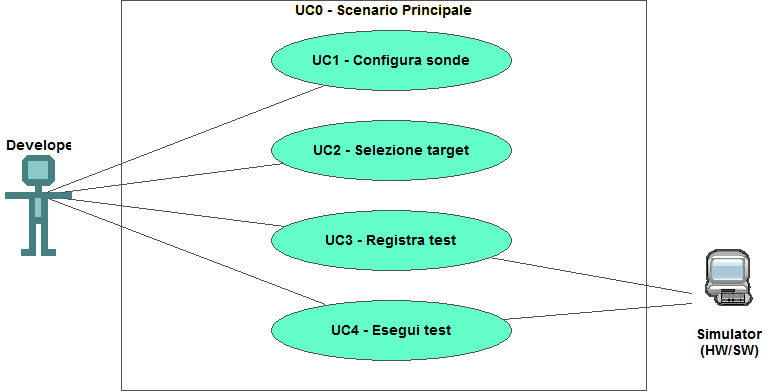
\includegraphics[width=0.9\columnwidth]{usecase/scenario-principale} 
    \caption{Use Case - UC0: Scenario principale}
\end{figure}

\begin{usecase}{0}{Scenario principale}
\usecaseactors{Sviluppatore applicativi}
\usecasepre{Lo sviluppatore è entrato nel plug-in di simulazione all'interno dell'IDE}
\usecasedesc{La finestra di simulazione mette a disposizione i comandi per configurare, registrare o eseguire un test}
\usecasepost{Il sistema è pronto per permettere una nuova interazione}
\label{uc:scenario-principale}
\end{usecase}

\section{Tracciamento dei requisiti}

Da un'attenta analisi dei requisiti e degli use case effettuata sul progetto è stata stilata la tabella che traccia i requisiti in rapporto agli use case.\\
Sono stati individuati diversi tipi di requisiti e si è quindi fatto utilizzo di un codice identificativo per distinguerli.\\
Il codice dei requisiti è così strutturato R(F/Q/V)(N/D/O) dove:
\begin{enumerate}
	\item[R =] requisito
    \item[F =] funzionale
    \item[Q =] qualitativo
    \item[V =] di vincolo
    \item[N =] obbligatorio (necessario)
    \item[D =] desiderabile
    \item[Z =] opzionale
\end{enumerate}
Nelle tabelle \ref{tab:requisiti-funzionali}, \ref{tab:requisiti-qualitativi} e \ref{tab:requisiti-vincolo} sono riassunti i requisiti e il loro tracciamento con gli use case delineati in fase di analisi.

\newpage

\begin{table}%
\caption{Tabella del tracciamento dei requisti funzionali}
\label{tab:requisiti-funzionali}
\begin{tabularx}{\textwidth}{lXl}
\hline\hline
\textbf{Requisito} & \textbf{Descrizione} & \textbf{Use Case}\\
\hline
RFN-1     & L'interfaccia permette di configurare il tipo di sonde del test & UC1 \\
\hline
\end{tabularx}
\end{table}%

\begin{table}%
\caption{Tabella del tracciamento dei requisiti qualitativi}
\label{tab:requisiti-qualitativi}
\begin{tabularx}{\textwidth}{lXl}
\hline\hline
\textbf{Requisito} & \textbf{Descrizione} & \textbf{Use Case}\\
\hline
RQD-1    & Le prestazioni del simulatore hardware deve garantire la giusta esecuzione dei test e non la generazione di falsi negativi & - \\
\hline
\end{tabularx}
\end{table}%

\begin{table}%
\caption{Tabella del tracciamento dei requisiti di vincolo}
\label{tab:requisiti-vincolo}
\begin{tabularx}{\textwidth}{lXl}
\hline\hline
\textbf{Requisito} & \textbf{Descrizione} & \textbf{Use Case}\\
\hline
RVO-1    & La libreria per l'esecuzione dei test automatici deve essere riutilizzabile & - \\
\hline
\end{tabularx}
\end{table}%             % Concept Preview
% !TEX encoding = UTF-8
% !TEX TS-program = pdflatex
% !TEX root = ../tesi.tex

%**************************************************************
\chapter{Progettazione e codifica}
\label{ch:progettazione-e-codifica}
%**************************************************************

\intro{In questo capitolo vengono presentate le tecnologie e gli strumenti utilizzati, il ciclo di sviluppo del software adottato e i design pattern utilizzati.}\\

%**************************************************************
\section{Tecnologie}
\label{sec:tecnologie}

Di seguito viene data una panoramica delle tecnologie e degli strumenti utilizzati.

\subsection*{CFR - decompilatore java}
CFR è il decompilatore utilizzato per trasformare il codice bytecode \textit{.class} in codice sorgente \textit{.java};
\url{http://www.benf.org/other/cfr/index.html}

\subsection*{Apk Tool}
Apktool è un tool per effettuare il reverse engineering delle applicazioni Android. Può decodificare le risorse contenute nell'APK in una forma quasi uguale a quelli originali, può anche di ricostruire l'APK dopo le modifiche alle risorse modificate.
\url{https://ibotpeaches.github.io/Apktool/}
\subsection*{Dex2Jar}
Questo strumento permette di trasformare i file \textit{.dex} in formato \textit{.jar} in modo che possa essere letta attraverso un software di compressione, come 7Zip, per poter accedere quindi ai file di tipo \textit{.class}.
\url{https://github.com/pxb1988/dex2jar}


\subsection*{Java}
In informatica, Java è un linguaggio di programmazione ad alto livello, orientato agli oggetti e tipizzazione statica, che si appoggia sull'omonima piattaforma software di esecuzione, specificamente progettato per essere il più possibile indipendente dalla piattaforma hardware di esecuzione.
\subsection*{Json}
JSON (JavaScript Object Notation) è un semplice formato per lo scambio di dati. Per le persone è facile da leggere e scrivere, mentre per le macchine risulta facile da generare e analizzarne la sintassi.
JSON è basato su due strutture:
\begin{itemize}
    \item un insieme di coppie nome/valore, in diversi linguaggi, questo è realizzato come un oggetto, un record, uno struct, un dizionario, una tabella hash, un elenco di chiavi o un array associativo.
    \item un elenco ordinato di valori, nella maggior parte dei linguaggi questo si realizza con un array, un vettore o una sequenza.
\end{itemize}
\url{https://www.json.org/json-it.html}
\section{Strumenti}\label{sec:strumenti}

\subsection*{Intellij IDEA}
L'IDE utilizzato per la scrittura del codice in Java sviluppato da JetBrains.
\url{https://www.jetbrains.com/idea/}

\subsection*{Android Emulator}
Lo strumento che permette di avviare degli emulatori Android, conosciuti anche come AVD. È stato utilizzato per eseguire l'applicazione ricompilata, per poter fare il dump dei dati presenti nell'area di storage dell'applicazione, come i file JSON, XML e SQLite, o come il file delle attività di rete.
\url{https://developer.android.com/studio/run/emulator}

\subsection*{Maven}
Maven è un tool di build automation, basato sul concetto di Project Object Model (POM), maven può gestire i build, fare il report e la documentazione da un singolo centro di informazione.
\url{https://maven.apache.org/}

\subsection*{Astah}
Astah è uno strumento di modellazione UML. Permette di creare vari diagrammi UML, come quelli di classe, di package, di sequenza e di attività.
\url{https://astah.net/products/astah-community/}

\subsection*{Git - GitLab}
Gitlab è una piattaforma web open-source che permette la gestione di repository e di funzioni d'issue tracking system.
Questa è un'istanza privata dell'azienda Imola Informatica S.p.A.
\url{https://git.imolinfo.it/users/sign_in}
%**************************************************************
\section{Ciclo di vita del software}\label{sec:ciclo-vita-software}

%**************************************************************
\section{Progettazione}
\label{sec:progettazione}

\subsection{Package}\label{subsec:package}
Questo è il root package del tool, contiene altri package e le due classi elencati successivamente.
\begin{namespacedesc}
    \classdesc{ApatLauncher}{È la classe di launcher del tool, si occupa principalmente di mettere in relazione di observed-observer i componenti della vista con i dati del modello;}
    \classdesc{Utils}{La classe di utilities che ha delle funzioni statiche utilizzata nel tool per evitare la ripetizione del codice.}
\end{namespacedesc}

\subsubsection{Package it.imolinfo.apat.controller} %**************************
Questo è il package che contiene la classe Controller e ciò che riguarda l'interazione del controller con il filesystem.
\begin{namespacedesc}
    \classdesc{AndroidManifestEditor.java}{È la classe che si occupa, dato un oggetto di tipo File Android Manifest, di modificare e/o aggiungere il tag \textit{debugabble} impostando il suo valore a \textit{true};}
    \classdesc{Controller}{È il controller del MVC, si occupa di effettuare le operazioni di decompilazione, ricompilazione, decodifica e analisi dei file;}
    \classdesc{MVCModule}{È la classe di effettuare la dependency injection per la creazione del MVC.}
\end{namespacedesc}

\subsubsection{Package it.imolinfo.apat.model} %**************************
Questo package contiene le classi che riguardano il modello del pattern Model View Controller.
\begin{namespacedesc}
    \classdesc{Modello}{La classe che contiene i dati utili al corretto funzionamento del tool;}
    \classdesc{ModelState}{È la classe che viene usato per poter salvare lo stato del funzionamento del tool. Lo stato viene salvato quando viene chiuso il tool, e viene ricaricato al successivo avvio;}
    \classdesc{PDFWriter}{È la classe wrapper che si occupa della creazione del file PDF per salvare i risultati dell'analisi;}
    \classdesc{Result}{È la classe di messaggio che viene restituita quando il tool interagisce con il file system;}
    \classdesc{Unzipper}{È la classe si occupa di decomprimere i file zip;}
    \classdesc{Dumper}{È la classe che si occupa di effettuare il dump dei dati da un file con estensione \textit{db};}
\end{namespacedesc}

\subsubsection{Package it.imolinfo.apat.pattern} %**************************
Questo package contiene degli sotto-package ognuno dei quali rappresenta un design pattern utilizzato nello sviluppo del tool.
I pattern utilizzati sono
\begin{namespacedesc}
    \classdesc{analyzer.Analyze}{È l'interfaccia di base del pattern Decorator.}
    \classdesc{analyzer.BaseAnalyze}{È la classe dell'oggetto base che viene decorato.}
    \classdesc{analyzer.BaseAnalyzeDecorator}{È il classe astratta del decorator di base che implementa l'interfaccia Analyze, e ha un metodo astratto \textit{doAnalysis()} che deve essere implementato dai decorator concreti.}
    \classdesc{analyzer.DumpDataBase}{È il decorator che si occupa di estrarre i contenuti dei file \textit{.db} scaricati dall'area di storage dell'app.}
    \classdesc{analyzer.DumpedFilesAnalyzer}{È il decorator che si occupa di analizzare i file dell'area di storage dell'applicazione con estensione \textit{XML} e \textit{json}, principalmente, legge il contenuto di tali file, e in base ad una whitelist, seleziona quali risultati restituire al chiamante.}
    \classdesc{analyzer.LambdaCounter}{È il decorator che conta il numero di lambda presente per ogni classe di codice \textit{.java} decompilato.}
    \classdesc{analyzer.StringFinder}{È il decorator che analizza i file di tipo \textit{.java}, ed estrae le stringhe hardcoded, può essere utilizzato insieme a un blacklist delle stringhe che devono essere ignorate.}
\end{namespacedesc}
\begin{namespacedesc}
    \classdesc{observer.Observable}{La classe parametrizzata T che può essere osservato;}
    \classdesc{observer.Observer}{L'interfaccia parametrizzata che ha il ruolo dell'observer;}
\end{namespacedesc}
\begin{namespacedesc}
    \classdesc{CliCommandFactory.Commands}{È l'interfaccia che contiene i metodi, dove ognuno dei quali deve generare delle istruzioni per la linea di comando.}
    \classdesc{CliCommandFactory.CommandFactory}{È la classe astratta che implementa la precendente interfaccia, con un costruttore di base che richiede un path di base.}
    \classdesc{CliCommandFactory.UnixCommandFactory}{È l'implementazione della classe astratta CommandFactory per il sistema UNIX.}
    \classdesc{CliCommandFactory.WindowsCommandFactory}{È l'implementazione della classe astratta CommandFactory per il sistema Windows.}
\end{namespacedesc}

\subsubsection{Package it.imolinfo.apat.view} %**************************
\begin{namespacedesc}
    \classdesc{AnalysisChooser}{È la finestra che mostra le opzioni di analisi.}
    \classdesc{View}{È la finestra principale, dove permette di selezionare il file \textit{apk} da decompilare ed analizzare.}
    \classdesc{WaitAction}{È una classe astratta che a sua volta eredita dalla classe Action e permette di eseguire un processo mostrando la barra del caricamento.}
    \classdesc{ApkFilter}{È l'implementazione dell'interfaccia \textbf{FileFilter} che accetta solo i file di tipo \textit{APK}.}
    \classdesc{KeyStoreFilter}{È l'implementazione dell'interfaccia \textbf{FileFilter} che accetta solo i file di tipo \textit{JKS}.}
    \classdesc{TextFilter}{È l'implementazione dell'interfaccia \textbf{FileFilter} che accetta solo i file di tipo \textit{txt}.}
\end{namespacedesc}


%**************************************************************

\section{Design Pattern utilizzati}\label{sec:design-pattern-utilizzati}
Di seguito, sono elencati i design pattern utilizzati durante la creazione del tool. Per ognuno di questo, verrà fornita il diagramma delle classi e una descrizione.
\subsection{Model View Controller}\label{subsec:model-view-controller}

\subsection{Observer}\label{subsec:observer}
Il pattern observer permette di definire una dipendenza uno a molti fra oggetti, in modo tale che se un oggetto cambia il suo stato, tutti gli oggetti dipendenti da questo siano notificati e aggiornati automaticamente.\\
Tale pattern viene applicato nel tool perché i componenti delle viste possano osservare il contenuto del modello.
\begin{figure}[H]
    \centering
    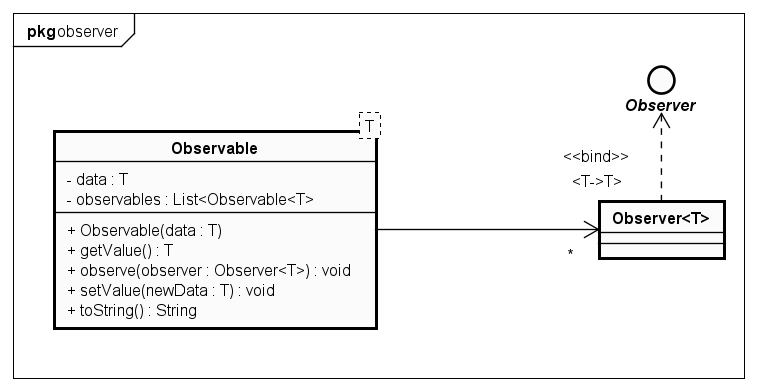
\includegraphics[width=14cm, height=8cm]{./immagini/diagrammi_uml/Observer.png}
    \caption{Diagramma delle classi del pattern Observer}\label{fig:observer}
\end{figure}
\subsection{Decorator}\label{subsec:decorator}
% todo descrivere il decorator
\begin{figure}[H]
    \centering
    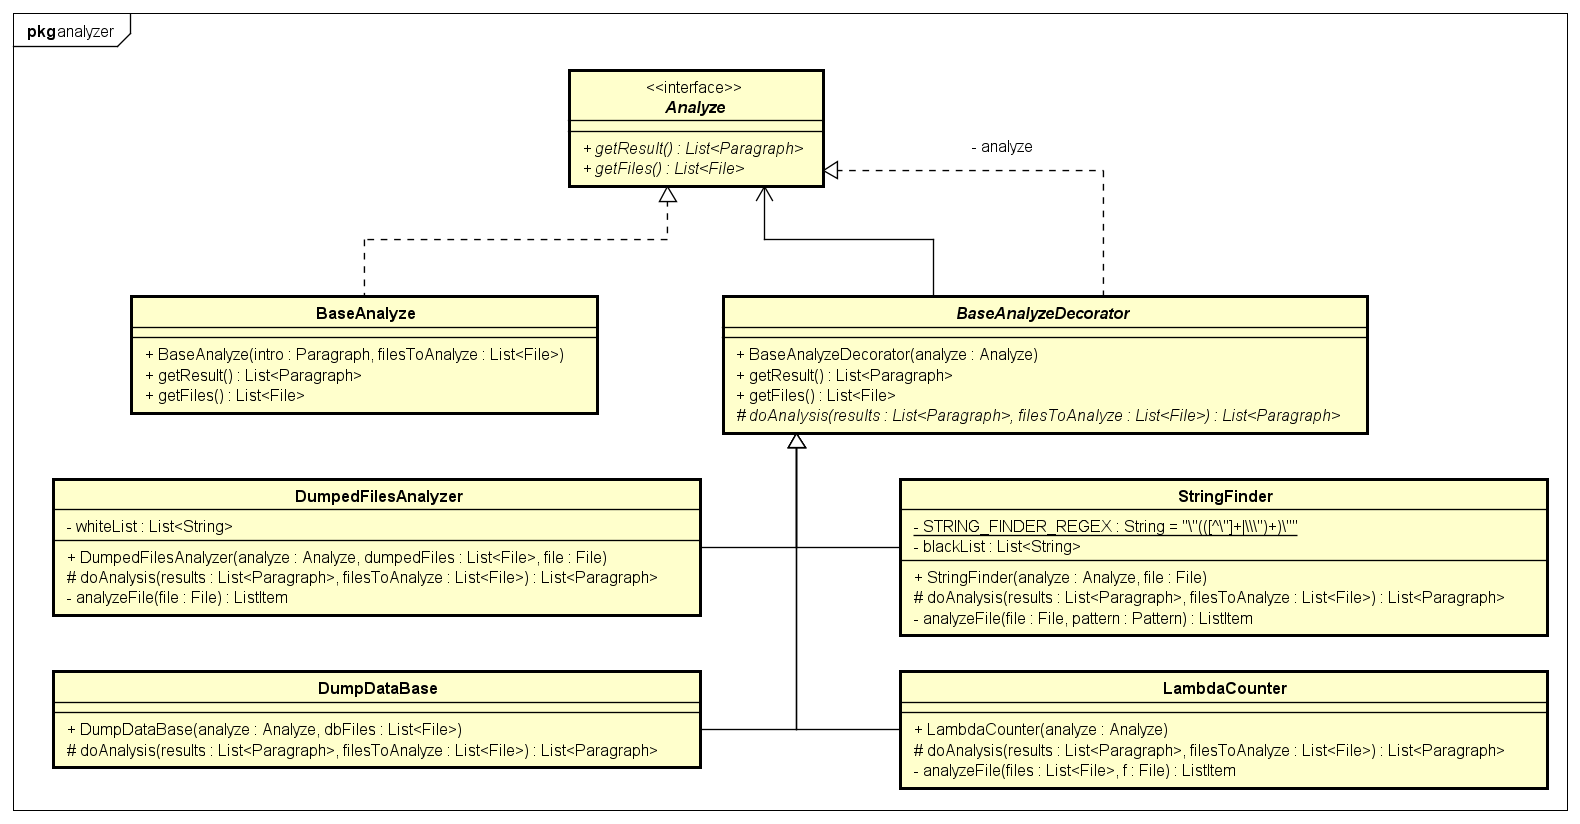
\includegraphics[width=14cm, height=10cm]{./immagini/diagrammi_uml/Decorator.png}
    \caption{Diagramma delle classi del pattern Decorator}\label{fig:decorator}
\end{figure}

\subsection{Factory Method}\label{subsec:factory-method}
% todo descrivere il factory method
\begin{figure}[H]
    \centering
    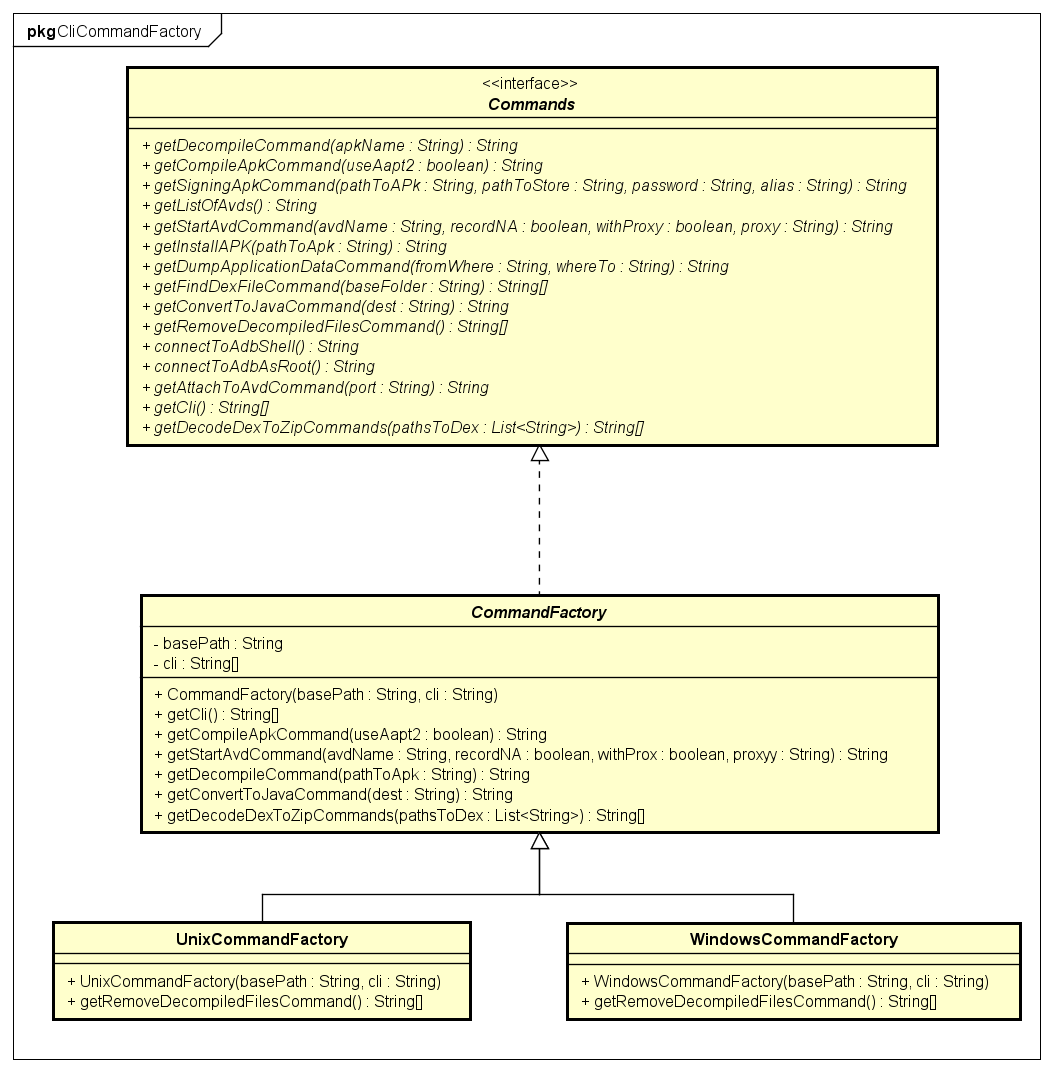
\includegraphics[width=14cm, height=12cm]{./immagini/diagrammi_uml/CommandFactory.png}
    \caption{Diagramma delle classi del pattern FactoryMethod}\label{fig:factory-method}
\end{figure}
%**************************************************************
\section{Codifica}\label{sec:codifica}
             % Product Prototype
% !TEX encoding = UTF-8
% !TEX TS-program = pdflatex
% !TEX root = ../tesi.tex

%**************************************************************
\chapter{Verifica e validazione}
\label{cap:verifica-validazione}
%**************************************************************             % Product Design Freeze e SOP
% !TEX encoding = UTF-8
% !TEX TS-program = pdflatex
% !TEX root = ../tesi.tex

%**************************************************************
\chapter{Conclusioni}
\label{ch:conclusioni}
%**************************************************************

%**************************************************************
\section{Consuntivo finale}\label{sec:consuntivo-finale}

%**************************************************************
\section{Raggiungimento degli obiettivi}\label{sec:raggiungimento-degli-obiettivi}

%**************************************************************
\section{Conoscenze acquisite}\label{sec:conoscenze-acquisite}

%**************************************************************
\section{Valutazione personale}\label{sec:valutazione-personale}
             % Conclusioni
\appendix
% !TEX encoding = UTF-8
% !TEX TS-program = pdflatex
% !TEX root = ../tesi.tex

%**************************************************************
\chapter{Appendice A}
%**************************************************************

\epigraph{Citazione}{Autore della citazione}



             % Appendice A

%**************************************************************
% Materiale finale
%**************************************************************
\backmatter
\printglossaries
% !TEX encoding = UTF-8
% !TEX TS-program = pdflatex
% !TEX root = ../tesi.tex

%**************************************************************
% Bibliografia
%**************************************************************

\cleardoublepage
\chapter{Bibliografia}\label{ch:bibliografia}

\nocite{*}
% Stampa i riferimenti bibliografici
\printbibliography[heading=subbibliography,title={Riferimenti bibliografici},type=book]

% Stampa i siti web consultati
\printbibliography[heading=subbibliography,title={Siti web consultati},type=online]


\end{document}
